% Options for packages loaded elsewhere
\PassOptionsToPackage{unicode}{hyperref}
\PassOptionsToPackage{hyphens}{url}
\documentclass[
  11pt,
]{report}
\usepackage{xcolor}
\usepackage[margin=2.5cm]{geometry}
\usepackage{amsmath,amssymb}
\setcounter{secnumdepth}{5}
\usepackage{iftex}
\ifPDFTeX
  \usepackage[T1]{fontenc}
  \usepackage[utf8]{inputenc}
  \usepackage{textcomp} % provide euro and other symbols
\else % if luatex or xetex
  \usepackage{unicode-math} % this also loads fontspec
  \defaultfontfeatures{Scale=MatchLowercase}
  \defaultfontfeatures[\rmfamily]{Ligatures=TeX,Scale=1}
\fi
\usepackage{lmodern}
\ifPDFTeX\else
  % xetex/luatex font selection
\fi
% Use upquote if available, for straight quotes in verbatim environments
\IfFileExists{upquote.sty}{\usepackage{upquote}}{}
\IfFileExists{microtype.sty}{% use microtype if available
  \usepackage[]{microtype}
  \UseMicrotypeSet[protrusion]{basicmath} % disable protrusion for tt fonts
}{}
\usepackage{setspace}
\makeatletter
\@ifundefined{KOMAClassName}{% if non-KOMA class
  \IfFileExists{parskip.sty}{%
    \usepackage{parskip}
  }{% else
    \setlength{\parindent}{0pt}
    \setlength{\parskip}{6pt plus 2pt minus 1pt}}
}{% if KOMA class
  \KOMAoptions{parskip=half}}
\makeatother
\usepackage{color}
\usepackage{fancyvrb}
\newcommand{\VerbBar}{|}
\newcommand{\VERB}{\Verb[commandchars=\\\{\}]}
\DefineVerbatimEnvironment{Highlighting}{Verbatim}{commandchars=\\\{\}}
% Add ',fontsize=\small' for more characters per line
\usepackage{framed}
\definecolor{shadecolor}{RGB}{248,248,248}
\newenvironment{Shaded}{\begin{snugshade}}{\end{snugshade}}
\newcommand{\AlertTok}[1]{\textcolor[rgb]{0.94,0.16,0.16}{#1}}
\newcommand{\AnnotationTok}[1]{\textcolor[rgb]{0.56,0.35,0.01}{\textbf{\textit{#1}}}}
\newcommand{\AttributeTok}[1]{\textcolor[rgb]{0.13,0.29,0.53}{#1}}
\newcommand{\BaseNTok}[1]{\textcolor[rgb]{0.00,0.00,0.81}{#1}}
\newcommand{\BuiltInTok}[1]{#1}
\newcommand{\CharTok}[1]{\textcolor[rgb]{0.31,0.60,0.02}{#1}}
\newcommand{\CommentTok}[1]{\textcolor[rgb]{0.56,0.35,0.01}{\textit{#1}}}
\newcommand{\CommentVarTok}[1]{\textcolor[rgb]{0.56,0.35,0.01}{\textbf{\textit{#1}}}}
\newcommand{\ConstantTok}[1]{\textcolor[rgb]{0.56,0.35,0.01}{#1}}
\newcommand{\ControlFlowTok}[1]{\textcolor[rgb]{0.13,0.29,0.53}{\textbf{#1}}}
\newcommand{\DataTypeTok}[1]{\textcolor[rgb]{0.13,0.29,0.53}{#1}}
\newcommand{\DecValTok}[1]{\textcolor[rgb]{0.00,0.00,0.81}{#1}}
\newcommand{\DocumentationTok}[1]{\textcolor[rgb]{0.56,0.35,0.01}{\textbf{\textit{#1}}}}
\newcommand{\ErrorTok}[1]{\textcolor[rgb]{0.64,0.00,0.00}{\textbf{#1}}}
\newcommand{\ExtensionTok}[1]{#1}
\newcommand{\FloatTok}[1]{\textcolor[rgb]{0.00,0.00,0.81}{#1}}
\newcommand{\FunctionTok}[1]{\textcolor[rgb]{0.13,0.29,0.53}{\textbf{#1}}}
\newcommand{\ImportTok}[1]{#1}
\newcommand{\InformationTok}[1]{\textcolor[rgb]{0.56,0.35,0.01}{\textbf{\textit{#1}}}}
\newcommand{\KeywordTok}[1]{\textcolor[rgb]{0.13,0.29,0.53}{\textbf{#1}}}
\newcommand{\NormalTok}[1]{#1}
\newcommand{\OperatorTok}[1]{\textcolor[rgb]{0.81,0.36,0.00}{\textbf{#1}}}
\newcommand{\OtherTok}[1]{\textcolor[rgb]{0.56,0.35,0.01}{#1}}
\newcommand{\PreprocessorTok}[1]{\textcolor[rgb]{0.56,0.35,0.01}{\textit{#1}}}
\newcommand{\RegionMarkerTok}[1]{#1}
\newcommand{\SpecialCharTok}[1]{\textcolor[rgb]{0.81,0.36,0.00}{\textbf{#1}}}
\newcommand{\SpecialStringTok}[1]{\textcolor[rgb]{0.31,0.60,0.02}{#1}}
\newcommand{\StringTok}[1]{\textcolor[rgb]{0.31,0.60,0.02}{#1}}
\newcommand{\VariableTok}[1]{\textcolor[rgb]{0.00,0.00,0.00}{#1}}
\newcommand{\VerbatimStringTok}[1]{\textcolor[rgb]{0.31,0.60,0.02}{#1}}
\newcommand{\WarningTok}[1]{\textcolor[rgb]{0.56,0.35,0.01}{\textbf{\textit{#1}}}}
\usepackage{longtable,booktabs,array}
\newcounter{none} % for unnumbered tables
\usepackage{calc} % for calculating minipage widths
% Correct order of tables after \paragraph or \subparagraph
\usepackage{etoolbox}
\makeatletter
\patchcmd\longtable{\par}{\if@noskipsec\mbox{}\fi\par}{}{}
\makeatother
% Allow footnotes in longtable head/foot
\IfFileExists{footnotehyper.sty}{\usepackage{footnotehyper}}{\usepackage{footnote}}
\makesavenoteenv{longtable}
\usepackage{graphicx}
\makeatletter
\newsavebox\pandoc@box
\newcommand*\pandocbounded[1]{% scales image to fit in text height/width
  \sbox\pandoc@box{#1}%
  \Gscale@div\@tempa{\textheight}{\dimexpr\ht\pandoc@box+\dp\pandoc@box\relax}%
  \Gscale@div\@tempb{\linewidth}{\wd\pandoc@box}%
  \ifdim\@tempb\p@<\@tempa\p@\let\@tempa\@tempb\fi% select the smaller of both
  \ifdim\@tempa\p@<\p@\scalebox{\@tempa}{\usebox\pandoc@box}%
  \else\usebox{\pandoc@box}%
  \fi%
}
% Set default figure placement to htbp
\def\fps@figure{htbp}
\makeatother
\setlength{\emergencystretch}{3em} % prevent overfull lines
\providecommand{\tightlist}{%
  \setlength{\itemsep}{0pt}\setlength{\parskip}{0pt}}
\usepackage{graphicx}
\usepackage{booktabs}
\usepackage{float}
\usepackage{amsmath,amssymb,amsthm}
\usepackage{caption}
\captionsetup{font=small}
\renewcommand{\thesection}{\arabic{section}}
\usepackage{bookmark}
\IfFileExists{xurl.sty}{\usepackage{xurl}}{} % add URL line breaks if available
\urlstyle{same}
\hypersetup{
  hidelinks,
  pdfcreator={LaTeX via pandoc}}

\author{}
\date{\vspace{-2.5em}}

\begin{document}

{
\setcounter{tocdepth}{2}
\tableofcontents
}
\setstretch{1.15}
\section{Insesgadez}\label{insesgadez}

\subsection{Definición}\label{definiciuxf3n}

Sea \(\hat{\theta}\) un estimador puntual de un parámetro \(\theta\). Se
dice que \(\hat{\theta}\) es un estimador insesgado si su valor esperado
coincide con el parámetro que pretende estimar:

\[E(\hat{\theta})=\theta\]

Equivalentemente, el sesgo se define como:

\[\operatorname{Sesgo}(\hat{\theta})
=
E(\hat{\theta})-\theta\]

Por consiguiente, un estimador es insesgado cuando:

\[\operatorname{Sesgo}(\hat{\theta})=0\]

\subsection{Interpretación}\label{interpretaciuxf3n}

La insesgadez indica que un estimador no tiende a sobreestimar ni
subestimar el parámetro poblacional. En promedio, las estimaciones
obtenidas a partir de muchas muestras coinciden con el valor real del
parámetro.

\subsection{Propiedad: Linealidad de la
Esperanza}\label{propiedad-linealidad-de-la-esperanza}

Una propiedad fundamental para demostrar la insesgadez es la linealidad
de la esperanza. Si \(X_1,X_2,\ldots,X_n\) son variables aleatorias y
\(a_1,a_2,\ldots,a_n\) son constantes, entonces:

\[E\left(
\sum_{i=1}^{n} a_i X_i
\right)
=
\sum_{i=1}^{n}
a_i E(X_i)\]

Esta propiedad permite demostrar que numerosos estimadores utilizados en
estadística son insesgados.

\subsection{Demostración de la insesgadez de la media
muestral}\label{demostraciuxf3n-de-la-insesgadez-de-la-media-muestral}

Sea:

\[\bar X
=
\frac{1}{n}
\sum_{i=1}^{n}
X_i\]

la media muestral de una muestra aleatoria simple.

Aplicando la linealidad de la esperanza:

\[E(\bar X)
=
E\left(
\frac{1}{n}
\sum_{i=1}^{n}
X_i
\right)\]

\[=
\frac{1}{n}
\sum_{i=1}^{n}
E(X_i)\]

Como cada observación tiene media poblacional \(\mu\):

\[E(X_i)=\mu\]

entonces:

\[E(\bar X)
=
\frac{1}{n}
(n\mu)
=
\mu\]

Por lo tanto:

\[E(\bar X)=\mu\]

lo que demuestra que la media muestral es un estimador insesgado de la
media poblacional.

\subsection{Insesgadez de la varianza muestral y corrección de
Bessel}\label{insesgadez-de-la-varianza-muestral-y-correcciuxf3n-de-bessel}

La estimación de la varianza poblacional presenta una dificultad
adicional respecto a la estimación de la media. Consideremos el
estimador:

\[S_n^2
=
\frac{1}{n}
\sum_{i=1}^{n}
(X_i-\bar X)^2\]

A primera vista, este estimador parece una elección natural para estimar
la varianza poblacional \((\sigma^2)\). Sin embargo, se demostrará que
es un estimador sesgado.

\subsubsection{Propiedad auxiliar}\label{propiedad-auxiliar}

Se cumple la siguiente identidad:

\[\sum_{i=1}^{n}
(X_i-\bar X)^2
=
\sum_{i=1}^{n}
(X_i-\mu)^2
-
n(\bar X-\mu)^2\]

Tomando esperanza en ambos lados:

\[E\left[
\sum_{i=1}^{n}
(X_i-\bar X)^2
\right]
=
E\left[
\sum_{i=1}^{n}
(X_i-\mu)^2
\right]
-
nE[(\bar X-\mu)^2]\]

\subsubsection{Cálculo del primer
término}\label{cuxe1lculo-del-primer-tuxe9rmino}

Como:

\[Var(X_i)=\sigma^2\]

entonces:

\[E[(X_i-\mu)^2]
=
\sigma^2\]

y por linealidad de la esperanza:

\[E\left[
\sum_{i=1}^{n}
(X_i-\mu)^2
\right]
=
n\sigma^2\]

\subsubsection{Cálculo del segundo
término}\label{cuxe1lculo-del-segundo-tuxe9rmino}

Recordando que:

\[Var(\bar X)
=
\frac{\sigma^2}{n}\]

se tiene:

\[E[(\bar X-\mu)^2]
=
\frac{\sigma^2}{n}\]

Por consiguiente:

\[nE[(\bar X-\mu)^2]
=
\sigma^2\]

\subsubsection{Resultado}\label{resultado}

Sustituyendo ambos resultados:

\[E\left[
\sum_{i=1}^{n}
(X_i-\bar X)^2
\right]
=
n\sigma^2-\sigma^2\]

\[=
(n-1)\sigma^2\]

Por lo tanto:

\[E(S_n^2)
=
E\left[
\frac{1}{n}
\sum_{i=1}^{n}
(X_i-\bar X)^2
\right]\]

\[=
\frac{1}{n}
(n-1)\sigma^2\]

es decir,

\[E(S_n^2)
=
\frac{n-1}{n}
\sigma^2\]

Como:

\[\frac{n-1}{n}
\neq
1\]

se concluye que:

\[E(S_n^2)
\neq
\sigma^2\]

y, por tanto, \((S_n^2)\) es un estimador sesgado de la varianza
poblacional.

\subsubsection{Corrección de Bessel}\label{correcciuxf3n-de-bessel}

Para eliminar el sesgo se introduce el estimador:

\[S^2
=
\frac{1}{n-1}
\sum_{i=1}^{n}
(X_i-\bar X)^2\]

Tomando esperanza:

\[E(S^2)
=
\frac{1}{n-1}
E\left[
\sum_{i=1}^{n}
(X_i-\bar X)^2
\right]\]

\[=
\frac{1}{n-1}
(n-1)\sigma^2\]

Por lo tanto:

\[E(S^2)
=
\sigma^2\]

Se concluye que \((S^2)\) es un estimador insesgado de la varianza
poblacional. El reemplazo de \((n)\) por \((n-1)\) en el denominador se
conoce como \textbf{corrección de Bessel} y compensa la pérdida de un
grado de libertad ocasionada por la estimación previa de la media
poblacional mediante \((\bar X)\).

\subsection{Evidencia empírica mediante
simulación}\label{evidencia-empuxedrica-mediante-simulaciuxf3n}

Para complementar la demostración teórica, se realizó una simulación con
\(B=10000\)(Número de repeticiones) y muestras aleatorias de tamaño
\((n=30)\), generadas a partir de una población con media poblacional
\((\mu=50)\) y desviación estándar \((\sigma=10)\).

Para cada muestra se calculó la media muestral, obteniéndose una
distribución de estimaciones del parámetro poblacional.

\begin{Shaded}
\begin{Highlighting}[]
\FunctionTok{library}\NormalTok{(pacman)}
\FunctionTok{p\_load}\NormalTok{(ggplot2)}

\FunctionTok{set.seed}\NormalTok{(}\DecValTok{123}\NormalTok{)}

\NormalTok{mu }\OtherTok{\textless{}{-}} \DecValTok{50}
\NormalTok{sigma }\OtherTok{\textless{}{-}} \DecValTok{10}

\NormalTok{n }\OtherTok{\textless{}{-}} \DecValTok{30}
\NormalTok{B }\OtherTok{\textless{}{-}} \DecValTok{10000}

\NormalTok{estimaciones }\OtherTok{\textless{}{-}} \FunctionTok{replicate}\NormalTok{(}
\NormalTok{  B,}
  \FunctionTok{mean}\NormalTok{(}\FunctionTok{rnorm}\NormalTok{(n, mu, sigma))}
\NormalTok{)}
\end{Highlighting}
\end{Shaded}

El promedio de las estimaciones simuladas fue:

\[\overline{\hat{\mu}}
=
50.01865\]

Dado que el verdadero valor del parámetro es:

\[\mu = 50\]

el sesgo empírico se estimó mediante:

\[\widehat{\operatorname{Sesgo}}
=
\overline{\hat{\mu}}-\mu\]

es decir,

\[\widehat{\operatorname{Sesgo}}
=
50.01865-50
=
0.01865\]

Este valor es muy próximo a cero, lo que indica que las estimaciones
obtenidas se encuentran centradas alrededor del parámetro poblacional.

Debe tenerse en cuenta que el sesgo empírico no es exactamente nulo
debido a la variabilidad inherente al proceso de simulación. Sin
embargo, al aumentar el número de repeticiones, dicho valor tiende a
aproximarse cada vez más a cero.

Por consiguiente, la simulación proporciona evidencia empírica
consistente con el resultado teórico:

\[E(\bar X)=\mu\]

confirmando la propiedad de insesgadez de la media muestral.

\subsection{Representación gráfica}\label{representaciuxf3n-gruxe1fica}

\begin{figure}
\centering
\pandocbounded{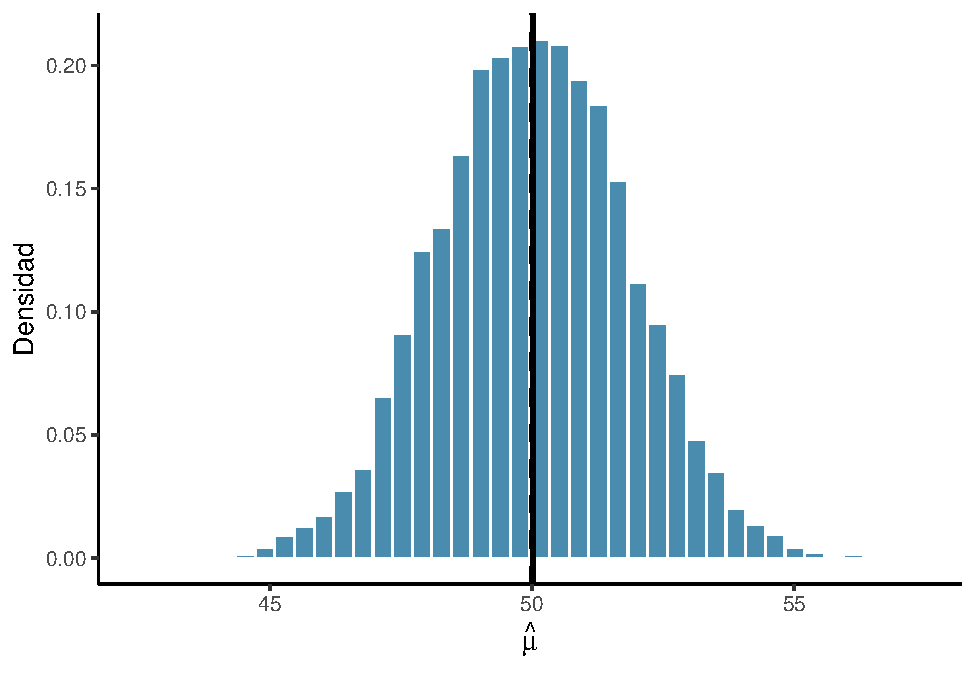
\includegraphics[keepaspectratio,alt={Distribución muestral de la media.}]{Estimadores-Puntuales_files/figure-latex/unnamed-chunk-2-1.pdf}}
\caption{Distribución muestral de la media.}
\end{figure}

La Figura muestra la distribución de las medias muestrales obtenidas
mediante simulación. La línea discontinua representa el valor verdadero
del parámetro poblacional \((\mu)\), mientras que la línea continua
corresponde al promedio de las estimaciones simuladas.

La proximidad entre ambas líneas proporciona evidencia visual de que la
media muestral constituye un estimador insesgado de la media
poblacional.

\textbf{Figura 1.} Distribución de las estimaciones obtenidas mediante
simulación. La coincidencia entre el parámetro verdadero y el promedio
de las estimaciones constituye evidencia de la ausencia de sesgo.

\subsection{Relación con el Error Cuadrático
Medio}\label{relaciuxf3n-con-el-error-cuadruxe1tico-medio}

El error cuadrático medio (ECM) se define como:

\[ECM(\hat{\theta})
=
E[(\hat{\theta}-\theta)^2]\]

y satisface la identidad:

\[ECM(\hat{\theta})
=
Var(\hat{\theta})
+
Sesgo^2(\hat{\theta})\]

Cuando el estimador es insesgado:

\[ECM(\hat{\theta})
=
Var(\hat{\theta})\]

Esta relación muestra que, una vez eliminado el sesgo, la variabilidad
del estimador se convierte en el principal criterio para evaluar su
calidad.

\subsection{Teorema de Rao-Blackwell}\label{teorema-de-rao-blackwell}

Una vez establecida la propiedad de insesgadez, surge el problema de
determinar si un estimador insesgado puede mejorarse sin perder dicha
propiedad.

El Teorema de Rao-Blackwell proporciona un procedimiento para construir
nuevos estimadores insesgados con menor variabilidad a partir de un
estimador inicial.

\subsubsection{Enunciado}\label{enunciado}

Sea \(\hat{\theta}\) un estimador insesgado de un parámetro \(\theta\) y
sea \(T(X)\) un estadístico suficiente para dicho parámetro.

Entonces:

\[\phi(T)
=
E(\hat{\theta}\mid T)\]

es también un estimador insesgado de \(\theta\) y satisface:

\[Var[\phi(T)]
\le
Var(\hat{\theta})\]

\subsubsection{Interpretación}\label{interpretaciuxf3n-1}

El teorema establece que la información contenida en un estadístico
suficiente puede utilizarse para construir un nuevo estimador que
conserve la propiedad de insesgadez y presente una variabilidad menor o
igual que la del estimador original.

Por lo tanto, el estimador obtenido mediante Rao-Blackwell aprovecha de
forma más eficiente la información disponible en la muestra.

\subsubsection{Consecuencias}\label{consecuencias}

Como resultado de este teorema se obtiene que:

\[E[\phi(T)]
=
\theta\]

por lo que la propiedad de insesgadez se preserva.

Además,

\[Var[\phi(T)]
\le
Var(\hat{\theta})\]

lo que implica una mejora en la precisión del estimador.

Dado que para estimadores insesgados se cumple:

\[ECM(\hat{\theta})
=
Var(\hat{\theta})\]

también se verifica que:

\[ECM[\phi(T)]
\le
ECM(\hat{\theta})\]

Por consiguiente, el procedimiento de Rao-Blackwell permite obtener
estimadores que mantienen la exactitud del estimador original y,
simultáneamente, reducen su error de estimación.

\subsubsection{Comentario}\label{comentario}

La aplicación formal de este resultado requiere el concepto de
estadístico suficiente y el Teorema de Factorización de Neyman-Fisher,
los cuales serán desarrollados en capítulos posteriores.

\begin{center}\rule{0.5\linewidth}{0.5pt}\end{center}

\section{Eficiencia}\label{eficiencia}

\subsection{Definición}\label{definiciuxf3n-1}

La eficiencia permite comparar estimadores insesgados de un mismo
parámetro.

Sean \(\hat{\theta}_1\) y \(\hat{\theta}_2\) dos estimadores insesgados
de \(\theta\). Se dice que \(\hat{\theta}_1\) es más eficiente que
\(\hat{\theta}_2\) si:

\[Var(\hat{\theta}_1)
<
Var(\hat{\theta}_2)\]

\subsection{Interpretación}\label{interpretaciuxf3n-2}

Mientras que la insesgadez evalúa la exactitud promedio de un estimador,
la eficiencia evalúa su precisión. Un estimador eficiente produce
estimaciones menos dispersas alrededor del parámetro verdadero.

\subsection{Justificación mediante el Error Cuadrático
Medio}\label{justificaciuxf3n-mediante-el-error-cuadruxe1tico-medio}

Si ambos estimadores son insesgados:

\[E(\hat{\theta}_1)
=
E(\hat{\theta}_2)
=
\theta\]

entonces:

\[ECM(\hat{\theta}_1)
=
Var(\hat{\theta}_1)\]

y

\[ECM(\hat{\theta}_2)
=
Var(\hat{\theta}_2)\]

Por lo tanto, entre dos estimadores insesgados, será preferible aquel
que posea menor varianza.

\subsection{Evidencia empírica mediante
simulación}\label{evidencia-empuxedrica-mediante-simulaciuxf3n-1}

Para ilustrar la eficiencia se comparan distribuciones muestrales de la
media calculadas con diferentes tamaños muestrales.

\begin{Shaded}
\begin{Highlighting}[]
\FunctionTok{set.seed}\NormalTok{(}\DecValTok{123}\NormalTok{)}

\NormalTok{theta }\OtherTok{\textless{}{-}} \DecValTok{50}
\NormalTok{sigma }\OtherTok{\textless{}{-}} \DecValTok{10}

\NormalTok{B }\OtherTok{\textless{}{-}} \DecValTok{5000}

\NormalTok{media\_n10 }\OtherTok{\textless{}{-}} \FunctionTok{replicate}\NormalTok{(}
\NormalTok{  B,}
  \FunctionTok{mean}\NormalTok{(}\FunctionTok{rnorm}\NormalTok{(}\DecValTok{10}\NormalTok{, theta, sigma))}
\NormalTok{)}

\NormalTok{media\_n50 }\OtherTok{\textless{}{-}} \FunctionTok{replicate}\NormalTok{(}
\NormalTok{  B,}
  \FunctionTok{mean}\NormalTok{(}\FunctionTok{rnorm}\NormalTok{(}\DecValTok{50}\NormalTok{, theta, sigma))}
\NormalTok{)}

\NormalTok{datos }\OtherTok{\textless{}{-}} \FunctionTok{data.frame}\NormalTok{(}
  \AttributeTok{valor =} \FunctionTok{c}\NormalTok{(media\_n10, media\_n50),}
  \AttributeTok{grupo =} \FunctionTok{factor}\NormalTok{(}
    \FunctionTok{rep}\NormalTok{(}\FunctionTok{c}\NormalTok{(}\StringTok{"n = 10"}\NormalTok{, }\StringTok{"n = 50"}\NormalTok{),}
        \AttributeTok{each =}\NormalTok{ B)}
\NormalTok{  )}
\NormalTok{)}
\end{Highlighting}
\end{Shaded}

Según la teoría:

\[Var(\bar X)
=
\frac{\sigma^2}{n}\]

Por lo tanto, al aumentar el tamaño muestral la varianza disminuye.

\subsection{Comparación mediante
densidades}\label{comparaciuxf3n-mediante-densidades}

\begin{Shaded}
\begin{Highlighting}[]
\FunctionTok{ggplot}\NormalTok{(}
\NormalTok{  datos,}
  \FunctionTok{aes}\NormalTok{(}
    \AttributeTok{x =}\NormalTok{ valor,}
    \AttributeTok{fill =}\NormalTok{ grupo,}
    \AttributeTok{color =}\NormalTok{ grupo}
\NormalTok{  )}
\NormalTok{) }\SpecialCharTok{+}
  \FunctionTok{geom\_density}\NormalTok{(}
    \AttributeTok{alpha =} \FloatTok{0.25}\NormalTok{,}
    \AttributeTok{linewidth =} \DecValTok{1}
\NormalTok{  ) }\SpecialCharTok{+}
  \FunctionTok{geom\_vline}\NormalTok{(}
    \AttributeTok{xintercept =}\NormalTok{ theta,}
    \AttributeTok{linetype =} \StringTok{"dashed"}\NormalTok{,}
    \AttributeTok{linewidth =} \DecValTok{1}
\NormalTok{  ) }\SpecialCharTok{+}
  \FunctionTok{scale\_fill\_manual}\NormalTok{(}
    \AttributeTok{values =} \FunctionTok{c}\NormalTok{(}\StringTok{"\#2978A0"}\NormalTok{, }\StringTok{"\#00B295"}\NormalTok{)}
\NormalTok{  ) }\SpecialCharTok{+}
  \FunctionTok{scale\_color\_manual}\NormalTok{(}
    \AttributeTok{values =} \FunctionTok{c}\NormalTok{(}\StringTok{"\#2978A0"}\NormalTok{, }\StringTok{"\#00B295"}\NormalTok{)}
\NormalTok{  ) }\SpecialCharTok{+}
  \FunctionTok{labs}\NormalTok{(}
    \AttributeTok{title =} \StringTok{"Comparación de eficiencia"}\NormalTok{,}
    \AttributeTok{x =} \FunctionTok{expression}\NormalTok{(}\FunctionTok{hat}\NormalTok{(theta)),}
    \AttributeTok{y =} \StringTok{"Densidad"}\NormalTok{,}
    \AttributeTok{fill =} \StringTok{""}\NormalTok{,}
    \AttributeTok{color =} \StringTok{""}
\NormalTok{  ) }\SpecialCharTok{+}
  \FunctionTok{theme\_classic}\NormalTok{(}\AttributeTok{base\_size =} \DecValTok{13}\NormalTok{)}
\end{Highlighting}
\end{Shaded}

\pandocbounded{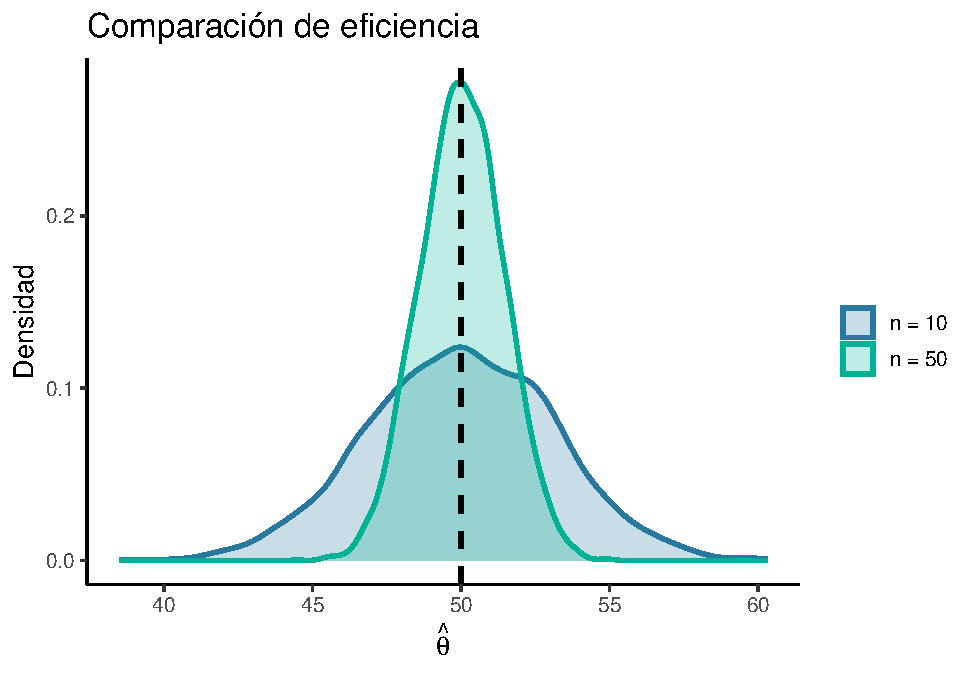
\includegraphics[keepaspectratio]{Estimadores-Puntuales_files/figure-latex/unnamed-chunk-4-1.pdf}}

\textbf{Figura 2.} Ambas distribuciones están centradas en el parámetro
verdadero, pero la correspondiente a \(n=50\) presenta una menor
dispersión, indicando una mayor eficiencia.

\subsection{Comparación mediante diagramas de
caja}\label{comparaciuxf3n-mediante-diagramas-de-caja}

\begin{Shaded}
\begin{Highlighting}[]
\FunctionTok{ggplot}\NormalTok{(}
\NormalTok{  datos,}
  \FunctionTok{aes}\NormalTok{(}
    \AttributeTok{x =}\NormalTok{ grupo,}
    \AttributeTok{y =}\NormalTok{ valor,}
    \AttributeTok{fill =}\NormalTok{ grupo}
\NormalTok{  )}
\NormalTok{) }\SpecialCharTok{+}
  \FunctionTok{geom\_boxplot}\NormalTok{(}
    \AttributeTok{alpha =} \FloatTok{0.85}
\NormalTok{  ) }\SpecialCharTok{+}
  \FunctionTok{geom\_hline}\NormalTok{(}
    \AttributeTok{yintercept =}\NormalTok{ theta,}
    \AttributeTok{linetype =} \StringTok{"dashed"}
\NormalTok{  ) }\SpecialCharTok{+}
  \FunctionTok{scale\_fill\_manual}\NormalTok{(}
    \AttributeTok{values =} \FunctionTok{c}\NormalTok{(}\StringTok{"\#2978A0"}\NormalTok{, }\StringTok{"\#00B295"}\NormalTok{)}
\NormalTok{  ) }\SpecialCharTok{+}
  \FunctionTok{labs}\NormalTok{(}
    \AttributeTok{title =} \StringTok{"Variabilidad de las estimaciones"}\NormalTok{,}
    \AttributeTok{x =} \StringTok{""}\NormalTok{,}
    \AttributeTok{y =} \FunctionTok{expression}\NormalTok{(}\FunctionTok{hat}\NormalTok{(theta))}
\NormalTok{  ) }\SpecialCharTok{+}
  \FunctionTok{theme\_classic}\NormalTok{(}\AttributeTok{base\_size =} \DecValTok{13}\NormalTok{) }\SpecialCharTok{+}
  \FunctionTok{theme}\NormalTok{(}
    \AttributeTok{legend.position =} \StringTok{"none"}
\NormalTok{  )}
\end{Highlighting}
\end{Shaded}

\pandocbounded{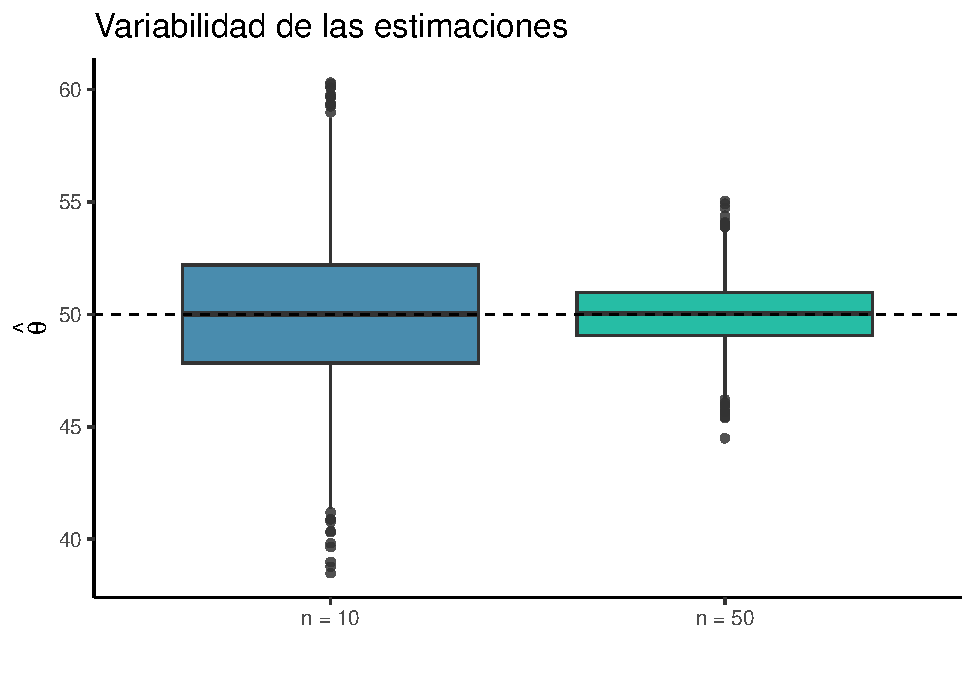
\includegraphics[keepaspectratio]{Estimadores-Puntuales_files/figure-latex/unnamed-chunk-5-1.pdf}}

\textbf{Figura 3.} La distribución asociada a un mayor tamaño muestral
presenta menor dispersión, lo que refleja una mayor eficiencia.

\subsection{Comparación numérica de
varianzas}\label{comparaciuxf3n-numuxe9rica-de-varianzas}

\begin{Shaded}
\begin{Highlighting}[]
\NormalTok{tabla\_varianzas }\OtherTok{\textless{}{-}} \FunctionTok{data.frame}\NormalTok{(}
  \AttributeTok{Estimador =} \FunctionTok{c}\NormalTok{(}
    \StringTok{"Media muestral (n = 10)"}\NormalTok{,}
    \StringTok{"Media muestral (n = 50)"}
\NormalTok{  ),}
  \AttributeTok{Varianza =} \FunctionTok{c}\NormalTok{(}
    \FunctionTok{var}\NormalTok{(media\_n10),}
    \FunctionTok{var}\NormalTok{(media\_n50)}
\NormalTok{  )}
\NormalTok{)}

\NormalTok{knitr}\SpecialCharTok{::}\FunctionTok{kable}\NormalTok{(}
\NormalTok{  tabla\_varianzas,}
  \AttributeTok{digits =} \DecValTok{4}\NormalTok{,}
  \AttributeTok{caption =} \StringTok{"Comparación de varianzas empíricas"}
\NormalTok{)}
\end{Highlighting}
\end{Shaded}

\begin{longtable}[]{@{}lr@{}}
\caption{Comparación de varianzas empíricas}\tabularnewline
\toprule\noalign{}
Estimador & Varianza \\
\midrule\noalign{}
\endfirsthead
\toprule\noalign{}
Estimador & Varianza \\
\midrule\noalign{}
\endhead
\bottomrule\noalign{}
\endlastfoot
Media muestral (n = 10) & 9.8504 \\
Media muestral (n = 50) & 1.9646 \\
\end{longtable}

Los resultados numéricos complementan la evidencia gráfica y permiten
verificar la disminución de la varianza al aumentar el tamaño muestral.

\subsection{Propiedad de mínima
varianza}\label{propiedad-de-muxednima-varianza}

Dentro de la clase de estimadores insesgados existe especial interés en
aquellos que presentan la menor varianza posible.

\[Var(\hat{\theta}^{*})
\le
Var(\hat{\theta})\]

para cualquier otro estimador insesgado \(\hat{\theta}\).

Esta propiedad motiva la búsqueda de estimadores óptimos en teoría de
estimación.

\subsection{Relación entre Insesgadez y Eficiencia: Cota de
Cramér-Rao}\label{relaciuxf3n-entre-insesgadez-y-eficiencia-cota-de-cramuxe9r-rao}

La eficiencia de un estimador insesgado no puede evaluarse únicamente
observando su varianza. Es necesario contar con una referencia teórica
que permita determinar qué tan cercana se encuentra dicha varianza al
mejor valor posible.

La Cota de Cramér-Rao establece que, bajo ciertas condiciones de
regularidad, la varianza de cualquier estimador insesgado de un
parámetro \(\theta\) satisface:

\[Var(\hat{\theta})
\ge
\frac{1}{I(\theta)}\]

donde \(I(\theta)\) representa la información de Fisher.

Esta desigualdad proporciona una cota inferior para la varianza de los
estimadores insesgados. En consecuencia, ningún estimador insesgado
puede poseer una varianza menor que dicho límite.

\subsection{Interpretación}\label{interpretaciuxf3n-3}

La información de Fisher mide la cantidad de información que contiene
una muestra respecto al parámetro desconocido. Cuanto mayor sea esta
información, menor podrá ser la varianza alcanzable por un estimador
insesgado.

Por tanto:

\[I(\theta)\uparrow
\quad\Longrightarrow\quad
\frac{1}{I(\theta)}\downarrow\]

lo que implica una mayor precisión en la estimación.

\subsection{Eficiencia Relativa}\label{eficiencia-relativa}

La eficiencia de un estimador insesgado puede expresarse como:

\[e(\hat{\theta})
=
\frac{\frac{1}{I(\theta)}}
     {Var(\hat{\theta})}\]

Cuando:

\[e(\hat{\theta})=1\]

el estimador alcanza exactamente la Cota de Cramér-Rao y se considera
eficiente en sentido óptimo.

Si:

\[0<e(\hat{\theta})<1\]

el estimador sigue siendo insesgado, pero no aprovecha toda la
información disponible en la muestra.

\subsubsection{Comentario}\label{comentario-1}

La Cota de Cramér-Rao constituye el principal criterio teórico para
evaluar la eficiencia de estimadores insesgados. Su demostración
requiere el estudio de la información de Fisher y será desarrollada en
un capítulo posterior.

\section{Suficiencia}\label{suficiencia}

Sea \(X_1, X_2, \ldots, X_n\) una muestra extraída de una población con
función de densidad \(f(x;\theta)\), y sea
\(T = T(X_1, X_2, \ldots, X_n)\) una estadística.

\hfill\break
Según Fisher, la estadística \(T = T(X_1, X_2, \ldots, X_n)\) es
suficiente para efectuar inferencias sobre el parámetro θ cuando T
``resume el conjunto de información relevante suministrada por la
muestra''. Ningún otro estimador definido con la misma muestra puede
suministrar información adicional respecto de θ.

\hfill\break
Los análisis estadísticos se realizan mediante una reducción o
condensación de la información contenida en la muestra. Esta
condensación o reducción lleva a cabo la estadística
\(T = T(X_1, X_2, \ldots, X_n)\) debe producirse sin pérdida de
información y en este sentido la suficiencia reclama la propiedad de que
la estad´sitica debe tener en relación a la no pérdida de información.

Para poder comprender mejor el alcance del concepto de suficiencia y sus
consecuencias, comenzamos estudiando de qué manera una estadística
genera una partición del espacio muestral de observación.

\[\mathcal{X}=\{(X_1,\ldots,X_n)\in \mathbb{R}^n \,/\, X_i \text{ es variable aleatoria};\ i=1,2,\ldots,n\}\]

\textbf{Ejemplo 1.} Sea \(X_1, X_2, X_3\) una muestra aleatoria extraída
de una población de Bernoulli \(B(1;p)\). Hallar las particiciones
inducidas por las estadísticas.

\[T_1=t_1(X_1,X_2,X_3)=\frac{\sum_{i=1}^{3} X_i}{3}
\qquad \text{y} \qquad
T_2=t_2(X_1,X_2,X_3)=\max\{X_1,X_2,X_3\}\]

\textbf{Solución:} Como \(X_i \sim B(1,p)\), entonces tenemos:

\[X_i=
\begin{cases}
1, & \text{si ocurre éxito con probabilidad } p,\\
0, & \text{si ocurre fracaso con probabilidad } 1-p=q,
\end{cases}
\qquad \forall i=1,2,3\]

Luego, el espacio muestral de observaciones generado por la muestra
aleatoria es:

\[\chi = \{(0;0;0), (0;0;1), (0;1;0), (1;0;0), (0;1;1), (1;0;1), (1;1;0), (1;1;1)\}\]

En la tabla siguiente se muestran los valores que alcanza cada una de
las dos estadísticas propuestas.

\[\begin{array}{|c|c|c|}
\hline
\text{Muestra} & T_1=t_1(X_1,X_2,X_3) & T_2=t_2(X_1,X_2,X_3) \\
\hline
(0,0,0) & 0 & 0 \\
(0,0,1) & \frac{1}{3} & 1 \\
(0,1,0) & \frac{1}{3} & 1 \\
(1,0,0) & \frac{1}{3} & 1 \\
(0,1,1) & \frac{2}{3} & 1 \\
(1,0,1) & \frac{2}{3} & 1 \\
(1,1,0) & \frac{2}{3} & 1 \\
(1,1,1) & 1 & 1 \\
\hline
\end{array}\]

\textbf{Tabla1.} Resultados de los estadíticos.

Así, la partición por \(T_1=t_1(X_1,X_2,X_3)\) está formada por los
siguientes subconjuntos:

\[\begin{matrix}
\chi_1 = \{(0;0;0)\}, & \chi_2 = \{(0;0;1), (0;1;0), (1;0;0)\} \\
\chi_3 = \{(0;1;1), (1;0;1), (1;1;0)\}, & \chi_4 = \{(1;1;1)\}
\end{matrix}\]

Análogamente, la partición inducida por \(T_2 = t_2(X_1; X_2; X_3)\)
está constituida por los siguientes dos subconjuntos.

\(\chi_1 = \{(0;0;0)\}, \quad \chi_2 = \{(0;0;1), (0;1;0), (1;0;0), (0;1;1), (1;0;1), (1;1;0), (1;1;1)\}\)

\subsection{Definición}\label{definiciuxf3n-2}

Sea \(X_1, X_2, \dots, X_n\) una muestra aleatoria extraída de una
población con función de densidad \(f(x;\theta)\).

Se dice que una estadística \(T = t(X_1, X_2, \ldots, X_n)\) es
suficiente para θ, si y sólo si la distribución condicional de
\(X = (X_1, X_2, \ldots, X_n)\) dado \(T = t(X_1, X_2, \ldots, X_n)\) es
independiente de θ, \(\forall \theta\), esto es:

\(P[\underline{X} = \u nderline{x} / T = t]\) no depende de θ.

La idea es que si uno conoce el valor de la estadística suficiente
\(T = t(X_1, X_2, \ldots, X_n)\) , entonces los valores muestrales así
solos no son necesarios para tomar deciciones acerca de θ; y esto es
verdaero, pues la distribución muestra dado el valor de la estadística
suficiente \(T=t\) no depende de θ. Uno no puede esperar para enterarse
de algo acerca de θ mediante los valores muestrales si su distribución
no depende de θ.

\textbf{Teorema 3.- (Criterio de Factorización Fisher-Neyman)}

Sea \(X_1, \dots, X_n\) una muestra aleatoria extraída de una población
con función de densidad \(f(x; \theta)\). La estadística
\(T = t(X_1, \dots, X_n)\) es suficiente para \(\theta\), si y sólo si,
existen funciones \(g_\theta\) y \(h\) tal que la densidad conjunta de
\(X_1, \dots, X_n\) se puede factorizar como

\[f(x_1, \dots, x_n; \theta) = g_\theta(t(x_1, \dots, x_n)) h(x_1, \dots, x_n) = g_\theta(T) h(x_1, \dots, x_n)\]

donde la función \(h(x_1, \dots, x_n)\) es no negativa y no depende del
parámetro \(\theta\), y la función \(g_\theta(t(x_1, \dots, x_n))\) es
no negativa y depende del parámetro \(\theta\) y de la muestra,
solamente a través de la estadística \(T = t(x_1, \dots, x_n)\).

\textbf{Teorema 4.- (Criterio de Factorización)}

Sea \(X_1, \dots, X_n\) una muestra aleatoria extraída de una población
con función de densidad de probabilidad \(f(x; \theta)\), donde
\(\underline{\theta} = (\theta_1, \dots, \theta_k) \in \Theta \subset \mathbb{R}^k\).
Una estadística m-dimensional

\[T = t(X_1, \dots, X_n) = (t_1(X_1, \dots, X_n), \dots, t_m(X_1, \dots, X_n)) = (T_1; T_2; \dots; T_m)\]

es suficiente para \(\underline{\theta}\), si y sólo si, la densidad
conjunta de \(X_1, \dots, X_n\) se factoriza como sigue

\[\begin{aligned}
f(x_1, \dots, x_n; \underline{\theta}) &= g_{\underline{\theta}}(t(x_1, \dots, x_n)) h(x_1, \dots, x_n) \\
&= g_{\underline{\theta}}((t_1(x_1, \dots, x_n), \dots, t_m(x_1, \dots, x_n))) h(x_1, \dots, x_n)
\end{aligned}\]

donde \(g_{\underline{\theta}}\) es una función no negativa y depende de
\(x_1, \dots, x_n\) sólo a través de \(T\) y \(h\) es una función
independiente de \(\theta\).

\textbf{Ejemplo 2.-} Sea \(X_1, \dots, X_n\) una muestra aleatoria
extraída de una población \(N(\mu; 1)\). Hallar una estadística
suficiente para \(\mu\).

\textbf{Solución:} La función de densidad de probabilidad de la
distribución \(N(\mu; 1)\) es dado por:

\[f(x; \mu) = \frac{1}{\sqrt{2\pi}} e^{-1/2(x-\mu)^2} = (2\pi)^{-1/2} \exp\left\{ -\frac{1}{2}(x^2 - 2\mu x + \mu^2) \right\}\]

Luego la densidad conjunta de la m.a. \(X_1, \dots, X_n\) es

\[\begin{aligned}
f(\underline{x}; \mu) &= \prod_{i=1}^n f(x_i; \mu) = \prod_{i=1}^n (2\pi)^{-1/2} \exp\left\{ -\frac{1}{2}x_i^2 + \mu x_i - \frac{1}{2}\mu^2 \right\} \\
&= (2\pi)^{-n/2} \exp\left\{ -\frac{1}{2}\sum x_i^2 + \mu \sum x_i - \frac{n\mu^2}{2} \right\} \\
&= (2\pi)^{-n/2} \exp\left\{ \mu \sum_{i=1}^n x_i - \frac{n\mu^2}{2} \right\} \cdot \exp\left\{ -\frac{1}{2}\sum_{i=1}^n x_i^2 \right\}
\end{aligned}\]

\[= (2\pi)^{-n/2} \exp\left\{ \mu T - \frac{n\mu^2}{2} \right\} \cdot \exp\left\{ -\frac{1}{2}\sum_{i=1}^n x_i^2 \right\} = g_\mu(T)h(\underline{x})\]

donde
\(h(\underline{x}) = \exp\left\{ -\frac{1}{2}\sum x_i^2 \right\} \quad ; \quad g_\mu(T) = \frac{1}{(2\pi)^{n/2}} \exp\left\{ \mu T - \frac{n}{2}\mu^2 \right\}\)

Por tanto, \(T = t(\underline{X}) = \sum_{i=1}^n X_i\) es una
estadística suficiente para \(\mu\).

\subsection{Implementación en R}\label{implementaciuxf3n-en-r}

Para ilustrar el resultado obtenido, se genera una muestra aleatoria de
una distribución Normal \(N(\mu,1)\) y se calcula la estadística
suficiente

\[T=\sum_{i=1}^{n}X_i.\]

\begin{Shaded}
\begin{Highlighting}[]
\CommentTok{\# Fijar semilla}
\FunctionTok{set.seed}\NormalTok{(}\DecValTok{123}\NormalTok{)}

\CommentTok{\# Parámetros}
\NormalTok{mu }\OtherTok{\textless{}{-}} \DecValTok{5}
\NormalTok{n }\OtherTok{\textless{}{-}} \DecValTok{20}

\CommentTok{\# Generar muestra aleatoria N(mu,1)}
\NormalTok{x }\OtherTok{\textless{}{-}} \FunctionTok{rnorm}\NormalTok{(n, }\AttributeTok{mean =}\NormalTok{ mu, }\AttributeTok{sd =} \DecValTok{1}\NormalTok{)}

\CommentTok{\# Estadística suficiente}
\NormalTok{T }\OtherTok{\textless{}{-}} \FunctionTok{sum}\NormalTok{(x)}

\CommentTok{\# Mostrar muestra}
\NormalTok{x}
\end{Highlighting}
\end{Shaded}

\begin{verbatim}
##  [1] 4.439524 4.769823 6.558708 5.070508 5.129288 6.715065 5.460916 3.734939
##  [9] 4.313147 4.554338 6.224082 5.359814 5.400771 5.110683 4.444159 6.786913
## [17] 5.497850 3.033383 5.701356 4.527209
\end{verbatim}

\begin{Shaded}
\begin{Highlighting}[]
\CommentTok{\# Mostrar estadística suficiente}
\NormalTok{T}
\end{Highlighting}
\end{Shaded}

\begin{verbatim}
## [1] 102.8325
\end{verbatim}

La estadística suficiente obtenida es:

\[T=\sum_{i=1}^{n}X_i.\]

De acuerdo con el Teorema de Factorización de Fisher-Neyman, toda la
información contenida en la muestra respecto al parámetro \(\mu\) queda
resumida en esta estadística.

\begin{verbatim}
\end{verbatim}

\begin{Shaded}
\begin{Highlighting}[]
\FunctionTok{library}\NormalTok{(ggplot2)}

\NormalTok{datos }\OtherTok{\textless{}{-}} \FunctionTok{data.frame}\NormalTok{(}\AttributeTok{x =}\NormalTok{ x)}

\FunctionTok{ggplot}\NormalTok{(datos, }\FunctionTok{aes}\NormalTok{(}\AttributeTok{x =}\NormalTok{ x)) }\SpecialCharTok{+}
  \FunctionTok{geom\_histogram}\NormalTok{(}\FunctionTok{aes}\NormalTok{(}\AttributeTok{y =} \FunctionTok{after\_stat}\NormalTok{(density)),}
                 \AttributeTok{bins =} \DecValTok{8}\NormalTok{,}
                 \AttributeTok{fill =} \StringTok{"skyblue"}\NormalTok{,}
                 \AttributeTok{color =} \StringTok{"black"}\NormalTok{,}
                 \AttributeTok{alpha =} \FloatTok{0.8}\NormalTok{) }\SpecialCharTok{+}
  \FunctionTok{geom\_density}\NormalTok{(}\AttributeTok{linewidth =} \FloatTok{1.2}\NormalTok{, }\AttributeTok{color =} \StringTok{"red"}\NormalTok{) }\SpecialCharTok{+}
  \FunctionTok{geom\_vline}\NormalTok{(}\AttributeTok{xintercept =}\NormalTok{ mu,}
             \AttributeTok{color =} \StringTok{"darkgreen"}\NormalTok{,}
             \AttributeTok{linewidth =} \FloatTok{1.2}\NormalTok{,}
             \AttributeTok{linetype =} \StringTok{"dashed"}\NormalTok{) }\SpecialCharTok{+}
  \FunctionTok{labs}\NormalTok{(}
    \AttributeTok{title =} \StringTok{"Muestra aleatoria de una distribución N(5,1)"}\NormalTok{,}
    \AttributeTok{subtitle =} \FunctionTok{paste}\NormalTok{(}\StringTok{"Estadística suficiente T ="}\NormalTok{, }\FunctionTok{round}\NormalTok{(T,}\DecValTok{2}\NormalTok{)),}
    \AttributeTok{x =} \StringTok{"Valores observados"}\NormalTok{,}
    \AttributeTok{y =} \StringTok{"Densidad"}
\NormalTok{  ) }\SpecialCharTok{+}
  \FunctionTok{theme\_classic}\NormalTok{(}\AttributeTok{base\_size =} \DecValTok{13}\NormalTok{)}
\end{Highlighting}
\end{Shaded}

\pandocbounded{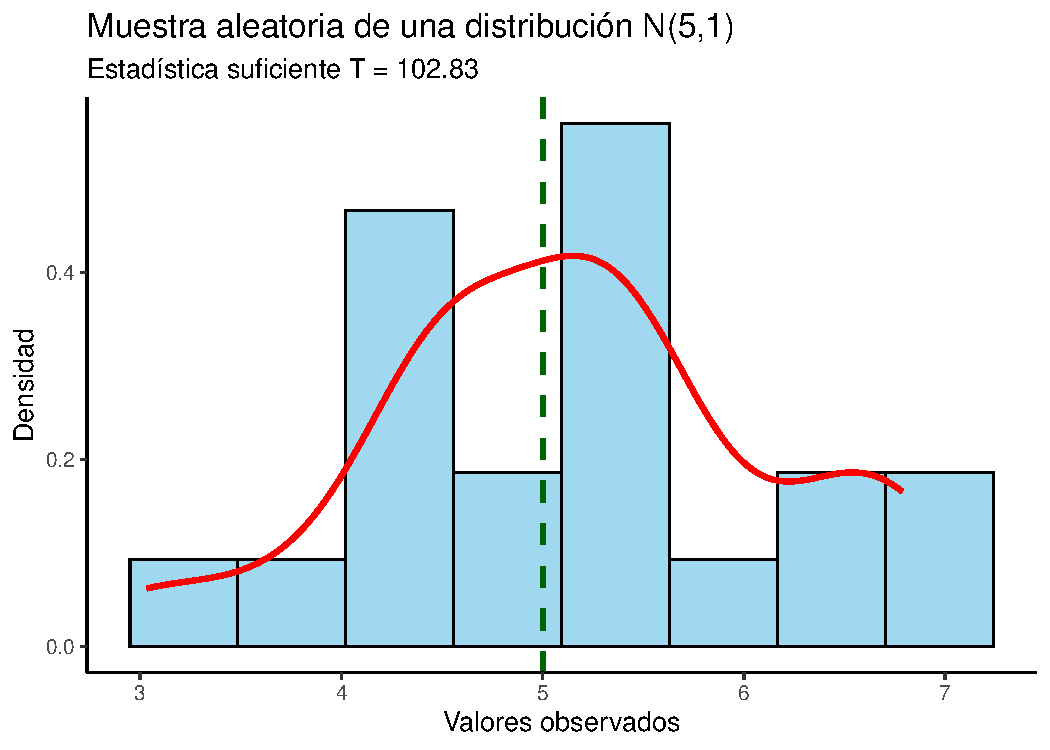
\includegraphics[keepaspectratio]{Estimadores-Puntuales_files/figure-latex/unnamed-chunk-8-1.pdf}}

\textbf{Figura4.} Distribución generada a partir de una población
\(N(5,1)\)

La figura muestra la distribución de la muestra generada a partir de una
población \(N(5,1)\). La línea vertical punteada representa la media
poblacional \(u=5\) . Para esta muestra, la estadística suficiente para
\(u\) es \(T=\sum_{i=1}^{n} X_i\), cuyo valor observado es \(T\).

\textbf{Ejemplo 3.-} Sea \(X_1, \dots, X_n\) una m.a. extraída de una
población \(N(\mu; \sigma^2)\) y sea
\(\underline{\theta} = (\mu; \sigma^2)\) el vector de parámetros. Hallar
una estadística suficiente para \(\underline{\theta}\).

\textbf{Solución:} La función conjunta de la muestra es:

\[\begin{aligned}
f(\underline{x}; \underline{\theta}) &= \prod_{i=1}^n f(x_i; \underline{\theta}) = \prod_{i=1}^n (2\pi)^{-1/2} \cdot \sigma^{-1} \cdot \exp\left\{ -\frac{1}{2\sigma^2}(x_i - \mu)^2 \right\} \\
&= (2\pi)^{-n/2} \cdot \sigma^{-n} \cdot \exp\left\{ -\frac{1}{2\sigma^2} \sum_{i=1}^n (x_i - \mu)^2 \right\} \\
&= \frac{1}{(2\pi)^{n/2} \cdot \sigma^n} \cdot \exp\left\{ -\frac{1}{2\sigma^2} \sum_{i=1}^n x_i^2 + \frac{\mu}{\sigma^2} \sum_{i=1}^n x_i - \frac{n\mu^2}{2\sigma^2} \right\} \\
&= \frac{1}{(2\pi)^{n/2} \cdot \sigma^n} \cdot \exp\left\{ -\frac{1}{2\sigma^2} T_2 + \frac{\mu}{\sigma^2} T_1 - \frac{n\mu^2}{2\sigma^2} \right\} = g_{\underline{\theta}}(T_1; T_2) h(\underline{x})
\end{aligned}\]

donde
\(h(\underline{x}) = 1 \quad ; \quad g_{\underline{\theta}}(T_1; T_2) = \frac{1}{(2\pi)^{n/2} \cdot \sigma^n} \cdot \exp\left\{ -\frac{1}{2\sigma^2} T_2 + \frac{\mu}{\sigma^2} T_1 - \frac{n\mu^2}{2\sigma^2} \right\}\)

Por tanto,
\(T = t(\underline{X}) = \left( \sum_{i=1}^n X_i ; \sum_{i=1}^n X_i^2 \right)\)
es una estadística suficiente para
\(\underline{\theta} = (\mu; \sigma^2)\)

Ejemplo3: Estadística suficiente para una población Normal

Sea \(X_1,\ldots,X_n\) una muestra aleatoria de una población

\[N(\mu,\sigma^2)\]

Aplicando el Teorema de Factorización de Fisher-Neyman se obtiene que

\[T(\mathbf{X})=
\left(
\sum_{i=1}^{n}X_i,
\sum_{i=1}^{n}X_i^2
\right)\]

es una estadística suficiente para el vector de parámetros

\[\boldsymbol{\theta}=(\mu,\sigma^2).\]

\subsection{Verificación mediante simulación en
R}\label{verificaciuxf3n-mediante-simulaciuxf3n-en-r}

\begin{Shaded}
\begin{Highlighting}[]
\CommentTok{\# Fijamos semilla para reproducibilidad}
\FunctionTok{set.seed}\NormalTok{(}\DecValTok{123}\NormalTok{)}

\CommentTok{\# Parámetros poblacionales}
\NormalTok{mu }\OtherTok{\textless{}{-}} \DecValTok{10}
\NormalTok{sigma }\OtherTok{\textless{}{-}} \DecValTok{2}
\NormalTok{n }\OtherTok{\textless{}{-}} \DecValTok{20}

\CommentTok{\# Generación de la muestra}
\NormalTok{x }\OtherTok{\textless{}{-}} \FunctionTok{rnorm}\NormalTok{(n, }\AttributeTok{mean =}\NormalTok{ mu, }\AttributeTok{sd =}\NormalTok{ sigma)}

\CommentTok{\# Estadísticas suficientes}
\NormalTok{T1 }\OtherTok{\textless{}{-}} \FunctionTok{sum}\NormalTok{(x)}
\NormalTok{T2 }\OtherTok{\textless{}{-}} \FunctionTok{sum}\NormalTok{(x}\SpecialCharTok{\^{}}\DecValTok{2}\NormalTok{)}

\CommentTok{\# Resultados}
\NormalTok{T1}
\end{Highlighting}
\end{Shaded}

\begin{verbatim}
## [1] 205.665
\end{verbatim}

\begin{Shaded}
\begin{Highlighting}[]
\NormalTok{T2}
\end{Highlighting}
\end{Shaded}

\begin{verbatim}
## [1] 2186.806
\end{verbatim}

La salida proporciona los valores observados de

\[T_1=\sum_{i=1}^{n}X_i\]

y

\[T_2=\sum_{i=1}^{n}X_i^2,\]

que constituyen una estadística suficiente para \((\mu,\sigma^2)\).

\begin{Shaded}
\begin{Highlighting}[]
\FunctionTok{library}\NormalTok{(ggplot2)}

\NormalTok{datos }\OtherTok{\textless{}{-}} \FunctionTok{data.frame}\NormalTok{(}
  \AttributeTok{i =} \DecValTok{1}\SpecialCharTok{:}\NormalTok{n,}
  \AttributeTok{x =}\NormalTok{ x}
\NormalTok{)}

\CommentTok{\# Cálculo de estadísticos suficientes}
\NormalTok{T1 }\OtherTok{\textless{}{-}} \FunctionTok{sum}\NormalTok{(x)}
\NormalTok{T2 }\OtherTok{\textless{}{-}} \FunctionTok{sum}\NormalTok{(x}\SpecialCharTok{\^{}}\DecValTok{2}\NormalTok{)}

\FunctionTok{ggplot}\NormalTok{(datos, }\FunctionTok{aes}\NormalTok{(}\AttributeTok{x =}\NormalTok{ i, }\AttributeTok{y =}\NormalTok{ x)) }\SpecialCharTok{+}
  \FunctionTok{geom\_point}\NormalTok{(}\AttributeTok{size =} \DecValTok{2}\NormalTok{, }\AttributeTok{color =} \StringTok{"steelblue"}\NormalTok{) }\SpecialCharTok{+}
  \FunctionTok{geom\_line}\NormalTok{(}\AttributeTok{color =} \StringTok{"gray60"}\NormalTok{, }\AttributeTok{alpha =} \FloatTok{0.6}\NormalTok{) }\SpecialCharTok{+}
  \FunctionTok{labs}\NormalTok{(}
    \AttributeTok{title =} \StringTok{"Muestra aleatoria de N(μ, σ²)"}\NormalTok{,}
    \AttributeTok{subtitle =} \FunctionTok{paste0}\NormalTok{(}\StringTok{"T1 = ΣXi = "}\NormalTok{, }\FunctionTok{round}\NormalTok{(T1,}\DecValTok{2}\NormalTok{),}
                      \StringTok{"   |   T2 = ΣXi² = "}\NormalTok{, }\FunctionTok{round}\NormalTok{(T2,}\DecValTok{2}\NormalTok{)),}
    \AttributeTok{x =} \StringTok{"Índice i"}\NormalTok{,}
    \AttributeTok{y =} \StringTok{"Valores de la muestra"}
\NormalTok{  ) }\SpecialCharTok{+}
  \FunctionTok{theme\_classic}\NormalTok{(}\AttributeTok{base\_size =} \DecValTok{13}\NormalTok{)}
\end{Highlighting}
\end{Shaded}

\pandocbounded{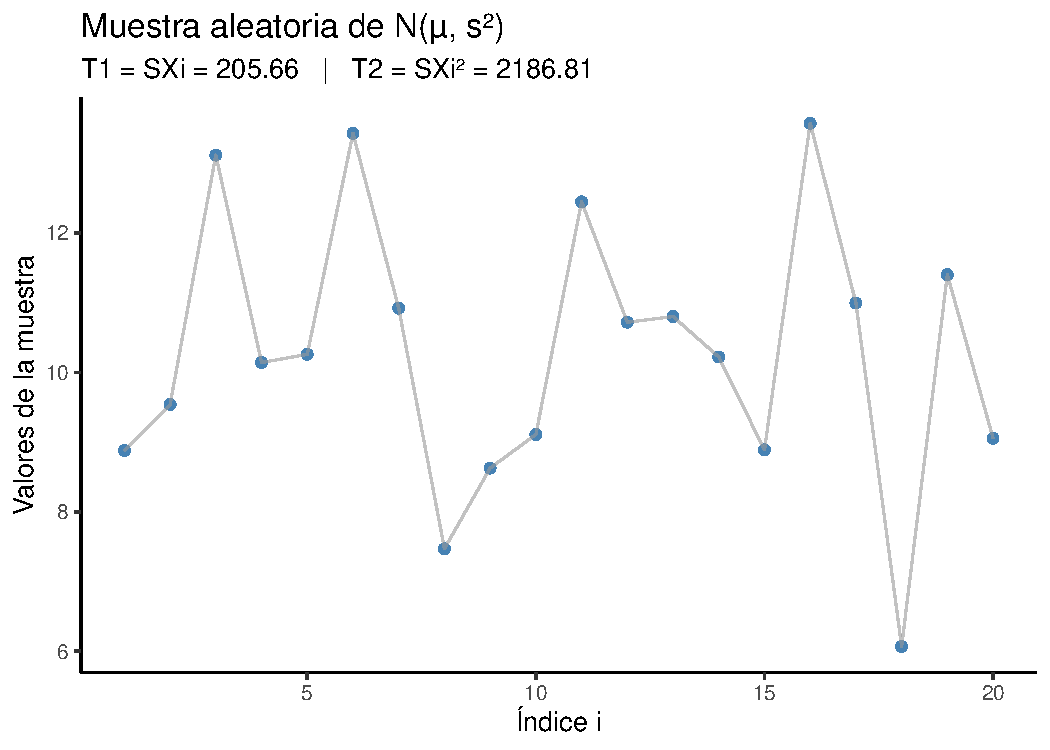
\includegraphics[keepaspectratio]{Estimadores-Puntuales_files/figure-latex/unnamed-chunk-10-1.pdf}}

Figura5.

EL gráfico muestra la muestra aleatoria generada de una población
\(N(\mu,\sigma^2)\). Toda la información relevante sobre los parámetros
\((\mu,\sigma^2)\) queda resumida en las estadísticas
suficientes\(T_1 = \sum X_i \text{ y } T_2 = \sum X_i^2\), lo que
confirma el resultado obtenido mediante el teorema de factorización de
Neyman-Fisher.

\section{Conclusiones}\label{conclusiones}

La muestra aleatoria proveniente de una población normal
\(N(\mu,\sigma^2)\) puede ser completamente resumida mediante la
estadística bidimensional \((T_1,T_2)=\left(\sum X_i,\sum X_i^2\right)\)
, la cual es suficiente para el vector de parámetros \((\mu,\sigma^2)\).
Esto implica que no se pierde información relevante sobre los parámetros
al reemplazar la muestra completa por estas estadísticas.

La existencia de una estadística suficiente para \((\mu,\sigma^2)\)
confirmar que la distribución normal pertenece a la familia exponencial,
lo que permite reducir la dimensionalidad de los datos sin afectar la
inferencia estadística. En particular, toda la información contenida en
la muestra sobre los parámetros se concentra en \(T_1 \text{ y } T_2\),
facilitando el cálculo de estimadores eficientes.

\section{Bibliografía}\label{bibliografuxeda}

\begin{itemize}
\tightlist
\item
  Mitacc Meza, M. \emph{Tópicos de inferencia estadística} (3.ª ed.).
  Lima, Perú.
\end{itemize}

\begin{itemize}
\tightlist
\item
  Moya, R. y Saravia, G. \emph{Probabilidad e inferencia estadística}.
  Perú.
\end{itemize}

\begin{itemize}
\tightlist
\item
  Huamani Flores, S. \emph{Apuntes de clase del curso: Análisis
  estadístico}. Material de curso, Perú.
\end{itemize}

\end{document}
